\begin{figure*}[!ht]
\begin{minipage}{.7\textwidth}
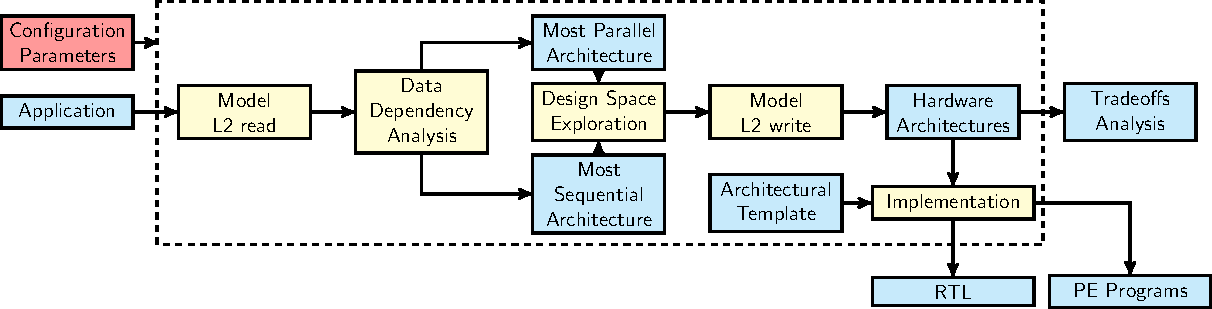
\includegraphics[width=\textwidth,left]{images/framework_v2.pdf}
  \caption{\small \frameworkname~Framework.}{}
  \label{fig:framework}
\end{minipage}%
\begin{minipage}{.3\textwidth}
    \centering
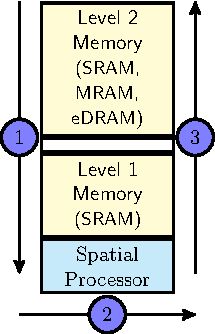
\includegraphics[width=.4\textwidth]{images/architecture_v2.pdf}
\caption{\small The system under analysis.
    }
\label{fig:system}
\end{minipage}
\squeezeup
\squeezeup
\end{figure*}
\section{The \frameworkname~framework}
\label{sec:framework}
The \frameworkname~framework, illustrated in Figure~\ref{fig:framework} takes two inputs, the \textit{Configuration Parameters} - described in Section~\ref{ssec:conf_param} - and an \textit{Application} - detailed in Section~\ref{ssec:app}, and automatically generates a set of hardware architectures, behaviorally equivalent to the input application.
%Ana: the sentence below was a repetition - can skip.
%Additionally, the analysis of area, power and latency of these architectures is automatically produced.
The generated hardware architectures can be realized as RTL implementations, using the \textit{architectural templates} described in Section~\ref{sec:arch_template}.
The rest of this section provides a detailed analysis of the design and implementation of \frameworkname.

\vspace{-1mm}
\subsection{Model of Execution}
\label{ssec:system_under_analysis}
\vspace{-1mm}
The system architecture we assume in this work has two levels of memory and a spatial processor (Figure~\ref{fig:system}). Level 1 memory (L1M)\footnotemark, the first memory level, and the smaller one in size, uses SRAM as it needs to be physically close to the processor for faster access. The second level - Level 2 memory (L2M)\footnotemark[\value{footnote}] - is larger in size and can be implemented using any memory technology (on-chip or off-chip), even with different access latency for read and write operations. Note that L2M can run at a different clock speed and different IO width than the processor and L1M.
\footnotetext{These memories are not to be seen as caches; thus, no cache policies are needed: we schedule data movements at design time. This is why we call them "levels" instead of "layers", and we abbreviate them with L1M and L2M instead of L1 and L2.}
We assume a model of execution following the three steps, from Figure~\ref{fig:system}, shown by arrows representing the direction of data flow. Initially, all the required input data for the application are available in L2M. The input data is transferred to the processor, using L1M as intermediate storage (step 1), the data is processed and the results are temporarily stored in L1M (step 2), and, finally, the data from L1M is transferred back to L2M (step 3). The data transfer between L2M and L1M are handled by a Direct Memory Access (DMA) controller. Note that our model of execution performs the steps in a pipelined manner, hence only part of the data will be stored in L1M at any given time.

\frameworkname~lets the user specify the parameters of the L2M through the \textit{Configuration Parameters}. The L2M parameters are used to model the data transfer between L2M and L1M (see \ref{ssec:layer2_model} and \ref{ssec:l2_read_model}). The L2M model is used to compute arrival time of input elements in the L1M. The arrival time of the element in the L1M is then used by the Modified Interval Partitioning (MIP) algorithm  - see \ref{ssec:modified_interval_partitioning}, to produce spatial architectures having bandwidth close to the bandwidth of the L2M. This effectively reduces the instantiation of unrequired resources in both the L1M and the spatial processor.
The L1M is composed of multiple banks having different depths. The number and depths of the banks composing the L1M is determined by the MIP as described in \ref{ssec:arch_tradeoffs}.

%Taking advantage of the possibility to produce stacked chip having levels produced using different manufacturing technologies we are able to explore different memory implementations at the L2 of the memory architecture.

%\begin{figure}[tb]
%\centering
%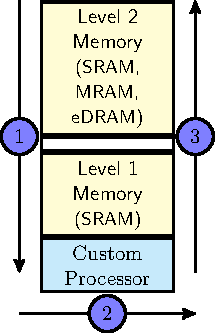
\includegraphics[width=0.25\columnwidth]{images/architecture.pdf}
%\caption{\small The system under analysis. Composed by two levels of memory, the memory at layer two can use various technologies while the memory at layer one uses only SRAM technology.}
%\label{fig:system}
%\end{figure}

\vspace{-1mm}
\subsection{The L2 Memory Model}
\label{ssec:layer2_model}
\vspace{-1mm}
Because L2M has higher access latency compared to the L1M and spatial processor, we model the L2M assuming its data is accessed in bursts.
%Figure~\ref{fig:l2model}  shows a representation of such access.
A read or write burst access to the L2M is controlled by a Direct Memory Access (DMA) controller, with the starting address and size of the burst given as input to the DMA. After an initial \textit{setup latency}, the accessed elements are transferred in sequence from the start address to the end address, from L1M to L2M in case of a write, and from L2M to L1M in case of a read.

\section{\frameworkname: Inputs}
This section details the two inputs of \frameworkname: the \textit{application} and the \textit{Configuration Parameters}.
\vspace{-1mm}
\subsection{Application}
\label{ssec:app}
\vspace{-1mm}
The applications that can be used as input to \frameworkname~are completely defined at compile time, having control-flow instructions not dependent on input data. Such applications enable the static extraction of data dependency information performed by the \textit{Data Dependency Analysis} module (\ref{ssec:dda}). We currently support C/C++ applications. However, as the framework uses the LLVM Intermediate Representation~\cite{llvm}, it can be easily extended to support other languages as well.
%\begin{lstlisting}[language=C, caption={Example of input application, C implementation of a matrix vector multiplication.}, label={lst:matrixvec}]
%void matrix_vec_kernel(int *A,int *B, int *C){
%    int sum;
%    for(int i=0;i<DIM2;i++){
%        sum=0;
%        for(int j=0;j<DIM1;j++){
%            sum+=A[i*DIM1+j]*B[j];
%        }
%        C[i]=sum;
%    }
%}
%\end{lstlisting}

\vspace{-1mm}
\subsection{Configuration Parameters}
\label{ssec:conf_param}
\vspace{-1mm}
The second input to the framework is a configuration file for the different building blocks to be used for hardware architecture realization. Through this file, the user can specify: different compute units (e.g. multipliers, adders), process technology to be used (e.g. 16nm, 28nm), the clock frequency of the processor and L1M, and the clock frequency L2M. Moreover, the user can specify the data-width used by the compute units, L1M and L2M.
Information to model the L2M burst accesses is also specified in this file: the setup latency for write/read accesses, the type of L2M to be used (e.g. MRAM, SRAM) and the size of the L2M. The different parameters in the configuration file are then used to access a database containing estimates (obtained by synthesis or from specs) of area usage, static and dynamic power, and latency of each of the building blocks. Our L1M implementation uses multiple memory banks of different sizes (see \ref{ssec:arch_tradeoffs}). To estimate the resource usage of the different types of these memories we built a linear model, using synthesis data. We compared the ability of our linear model to predict area, latency and power consumption against the data generated using the synthesis tool and we found it to be accurate - less then 2\% error in the area and static energy model and less than 28\% error in the dynamic energy model.

%\begin{lstlisting}[language=json, caption={Example of input configuration file}, label={lst:conf_file}]
%{
%   "resource_database": {
%	"technology": 16,
%	"clock_frequency": 1000,
%	"bitwidth_adder": 128,
%	"bitwidth_multiplier": 64,
%	"bitwidth_register_file": 128,
%	"type_l2": "tt1v1v85c",
%	"technology_l2": 16,
%	"clock_l2": 800,
%	"bitwidth_l2": 32,
%	"depth_l2":2048,
%	"setup_write_latency_l2":2,
%	"setup_read_latency_l2":2
%   }
%}
%
%\end{lstlisting}

\section{\frameworkname: Analysis}
This section describes the parts of the framework involved in modeling the data transfers between L2M and L1M, \textit{Model L2 read} and \textit{Model L2 write} (\ref{ssec:l2_read_model}),the modules that perform data dependence analysis, \textit{Data Dependency Analysis}(\ref{ssec:dda}), and the scheduling of the application operations (\ref{ssec:modified_interval_partitioning}).
\vspace{-1mm}
\subsection{L2 Memory Read and Write Modeling}
\label{ssec:l2_read_model}
\vspace{-1mm}
The first operation performed by the framework is to compute the transfer time of the application's input data from L2M to L1M, implemented in the \textit{Model L2 read} block of Figure \ref{fig:framework}. Using static analysis, we obtain details regarding the data structures used in the application. For example, in a matrix vector multiplication kernel, the static analysis extracts information about three data structures: an input matrix and an input vector, containing the input elements of the computation, and an output vector containing the output elements of the computation. An address in L2M is given to each input element used by the application; different data structures are placed in consecutive memory addresses. The entire data transfer is modeled as a single burst-read operation from L2M. The information required to compute the arrival clock cycle of each input element to L1M is extracted from the \textit{Configuration Parameters}.
Using this information, the exact clock at which each input element arrives in L1M can be computed as seen in (1). The equation symbols are described in Table~\ref{table:equation}.

\begin{equation}
AClk_i = S_r + R_{L2M} * (Add_{L2Mi}+1) * \frac{B_{L1M}}{B_{L2M}} * \frac{Clk_{L1M}}{Clk_{L2M}}
\end{equation}

\begin{table}[]
\centering
\footnotesize
\begin{tabular}{|l|l|}
\hline
\textbf{Symbol} & \textbf{Definition}                                           \\ \hline
$AClk_i$           & Clock at which element i arrives to L1M                \\
$S_r$             & Setup Latency of a L2M burst read                          \\
$R_{L2M}$       & L2M read latency (per read), in L2M clock cycles   \\
$Add_{L2Mi}$     & Offset of element i in the burst access \\
$B_{L1M}$        & Data bitwidth of L1M                                       \\
$B_{L2M}$        & Data bitwidth of L2M                                       \\
$Clk_{L1M}$      & Clock Frequency of L1M                                     \\
$Clk_{L2M}$      & Clock Frequency of L2M                                     \\
$WBL_{L2M}$      & L2M write burst latency                                    \\
$S_w$             & Setup Latency of a L2M burst write                         \\
$W_{L2M}$       & L2M write latency (per write) in L2M clock cycles  \\
$O$                 & Total number of output elements                            \\ \hline
\end{tabular}
\caption{\small Definition of symbols used in the equations}
\label{table:equation}
\end{table}
The schedule produced by the Modified Interval Partitioning (MIP), discussed in \ref{ssec:modified_interval_partitioning}, uses the arrival clock cycle computed in this phase to determine when each input element will be available for computation in L1M. The latency of the MIP schedule includes therefore the L2M$\rightarrow$L1M transfer, and the computation; it does not take into account the L1M$\rightarrow$L2M transfer of the results (phase 3 in Figure~\ref{fig:system}).
The \textit{Model L2 write} block in Figure \ref{fig:framework} computes the latency of the L1M$\rightarrow$L2M transfer. The MIP computes the clock cycle at which computation ends (phase 2 in Figure~\ref{fig:system}) and the last data item is written in L1M. The L1M$\rightarrow$L2M transfer can start immediately after the last output is generated.
The latency of the L1M$\rightarrow$L2M transfer is calculated using (2),
\begin{equation}
    WBL_{L2M} = S_w + W_{L2M} * O * \frac{B_{L2M}}{B_{L1M}} * \frac{Clk_{L1M}}{Clk_{L2M}}
\end{equation}
where the symbols have been defined in Table~\ref{table:equation}.


\vspace{-1mm}
\subsection{Data Dependency Analysis}
\label{ssec:dda}
\vspace{-1mm}
The \textit{Data Dependency Analysis (DDA)} module operates in three stages. The first two stages are the extraction of the \textit{Data Dependency Graph} (DDG)\cite{isoda1983global} from the application and the schedule of the DDG using the As Soon As Possible (ASAP) and As Late As Possible (ALAP) methodologies. These two steps are core elements in the analysis of high level code for hardware design\cite{hwang1991formal}. Finally, the third step (see \ref{ssec:modified_interval_partitioning}) maps DDG instructions to hardware components - or PEs - using a modified \textit{Interval Partitioning} algorithm~\cite{greedyIntervalPartitioning}.
%This next paragraph might be replaced with a reference

To extract the DDG from an application, we use LLVM  and custom transformations. We first convert the input application code to its LLVM Intermediate Representation. We then transform the code into static single assignment (SSA) form and perform full-loop unrolling on all of the application loops. After these transformations, there will be no control flow instructions in the application body, and each variable will be defined only once. It is now possible to follow the definition and use chain of the variables to produce a Data Dependency Graph like the one shown in Figure~\ref{fig:ddg}. The DDG represents each operation as a node - in Figure~\ref{fig:ddg} the input and output nodes represent respectively load and store instructions, while oval nodes represent computations - and each edge represents a dependency between operations.

We further process the obtained DDG, aiming to reduce the length of the path between the input nodes and the output nodes. This additional transformation is important because the length of these paths is equivalent to the number of sequential operations required to obtain the outputs, which in turn determines the latency of the application. Taking advantage of operation associativity (where possible) we can transform a long sequence of operations - like the one highlighted in Figure~\ref{fig:ddg} - into an equivalent shorter tree.
%\begin{figure}[ht]
%\begin{minipage}{.5\textwidth}
%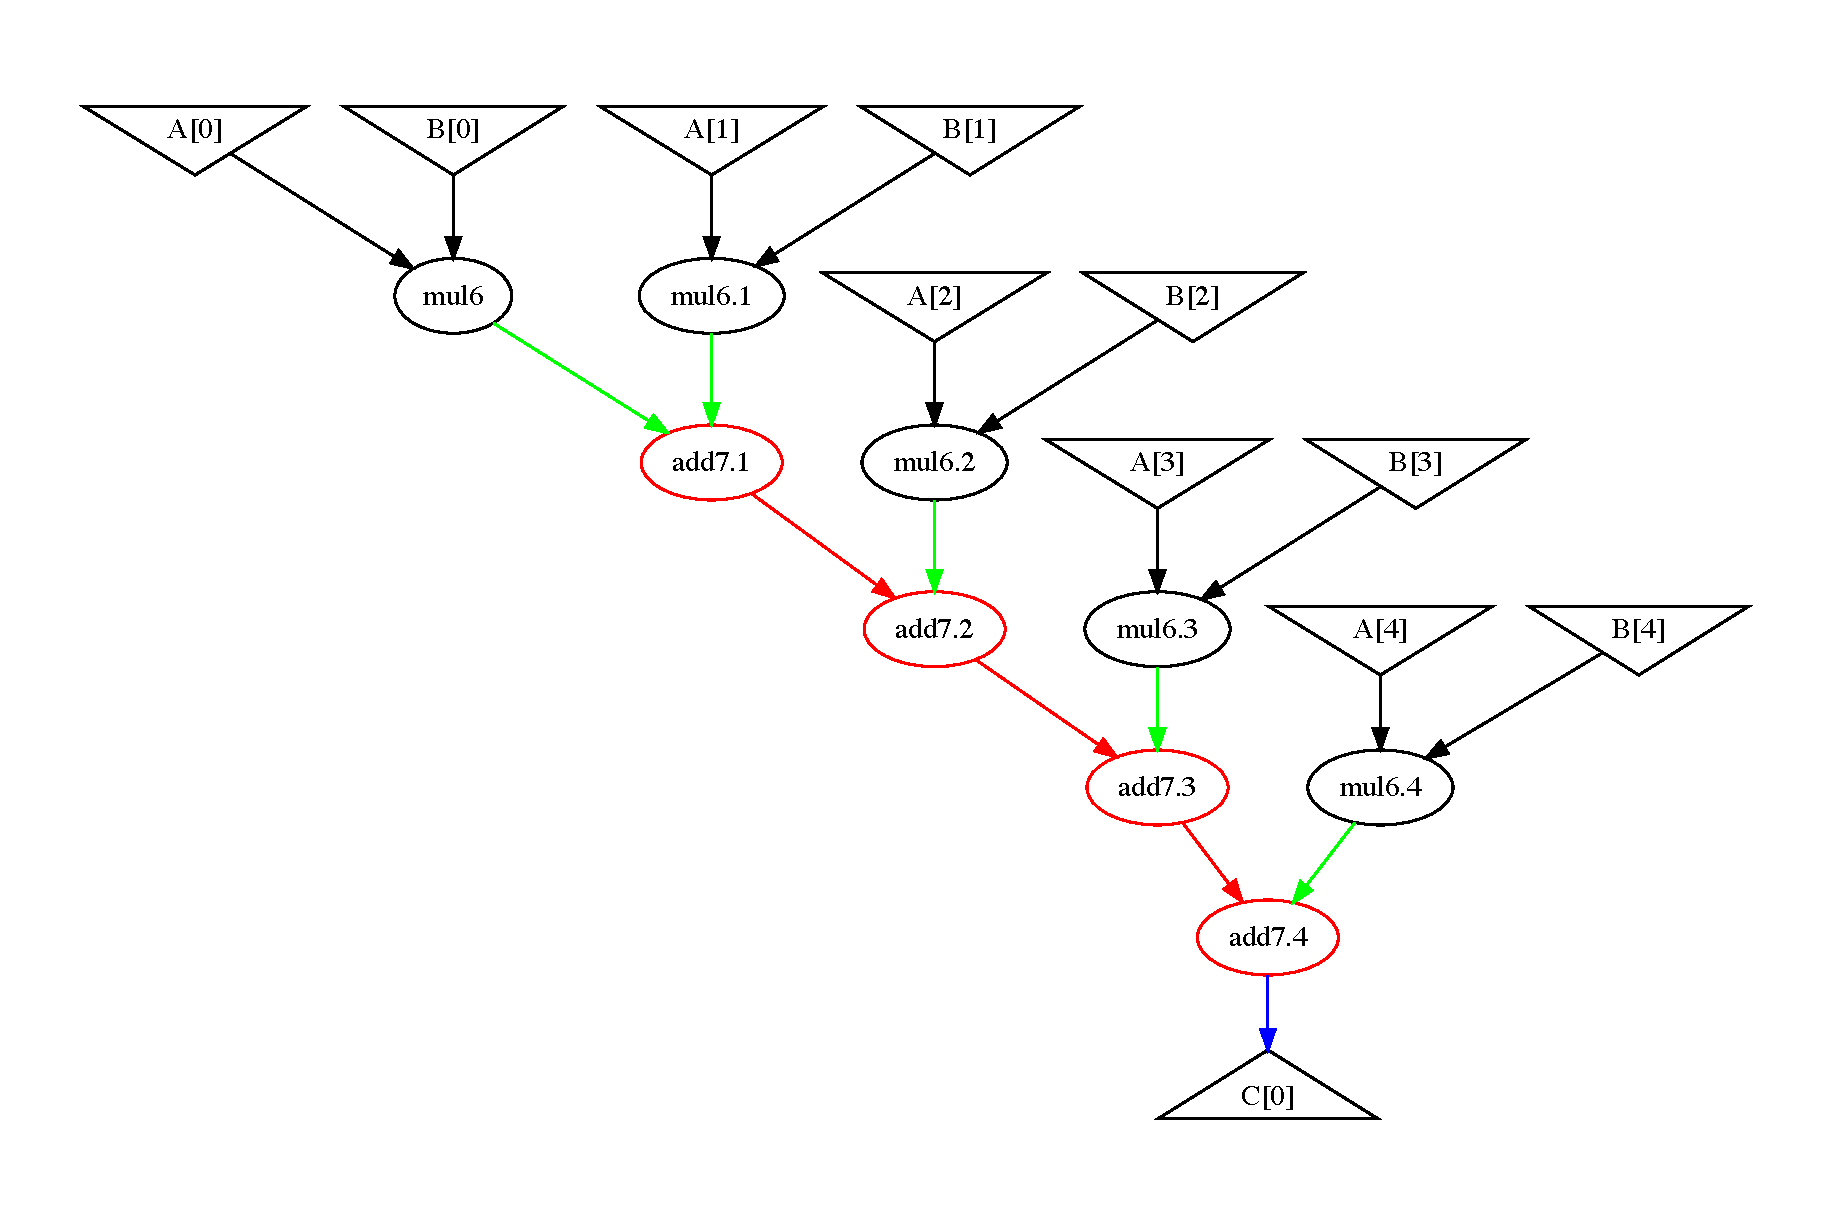
\includegraphics[width=.9\textwidth,left]{images/supernode.pdf}
%  \caption{\small \frameworkname~Framework.}{}
%  \label{fig:framework}
%\end{minipage}%
%\begin{minipage}{.5\textwidth}
%    \centering
%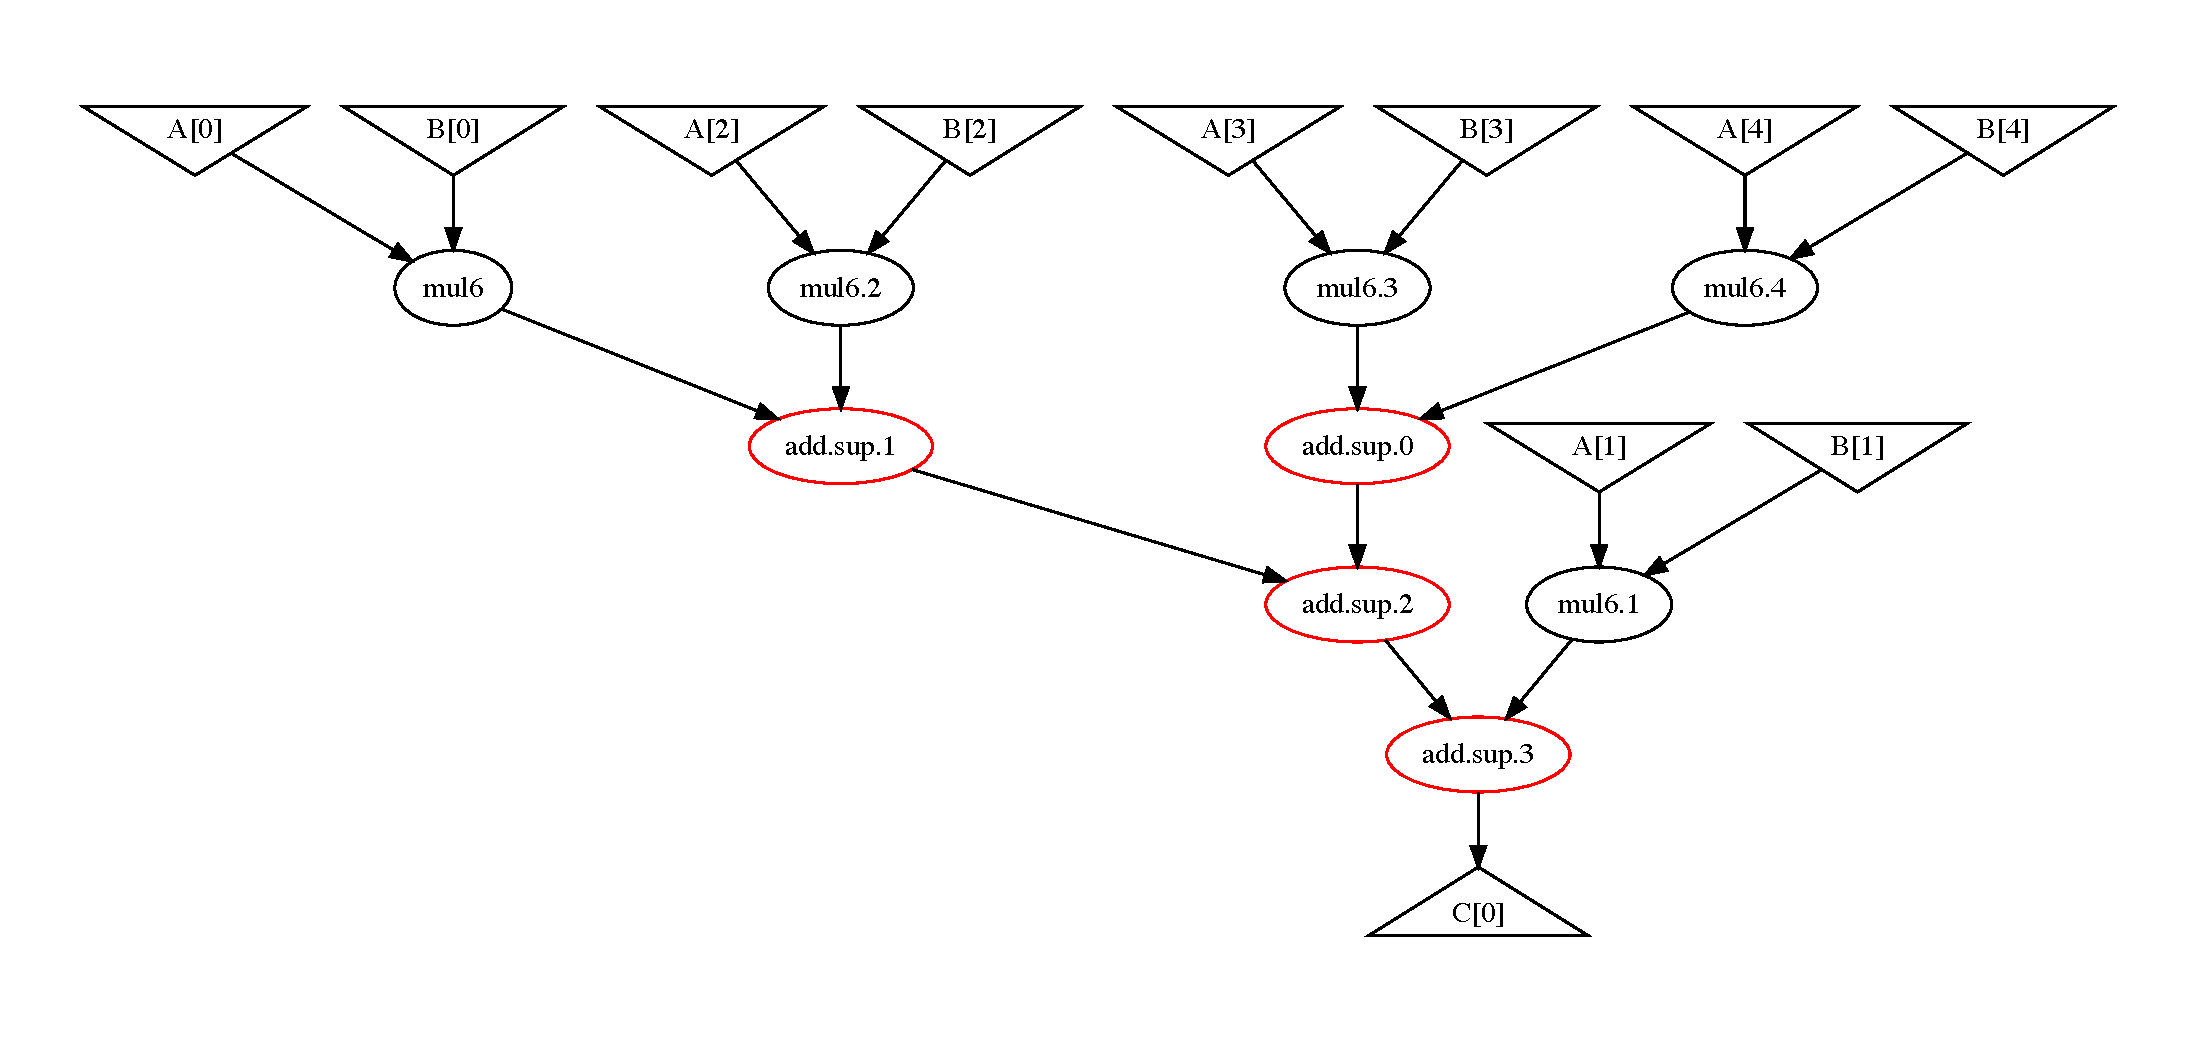
\includegraphics[width=.9\textwidth]{images/supernode_optimized.pdf}
%\caption{\small The system under analysis.
%    %Composed by two levels of memory, the memory at layer two can use various technologies while the memory at layer one uses only SRAM technology.
%    }
%\label{fig:system}
%\end{minipage}
%\end{figure}

\begin{figure}[tb]
\centering
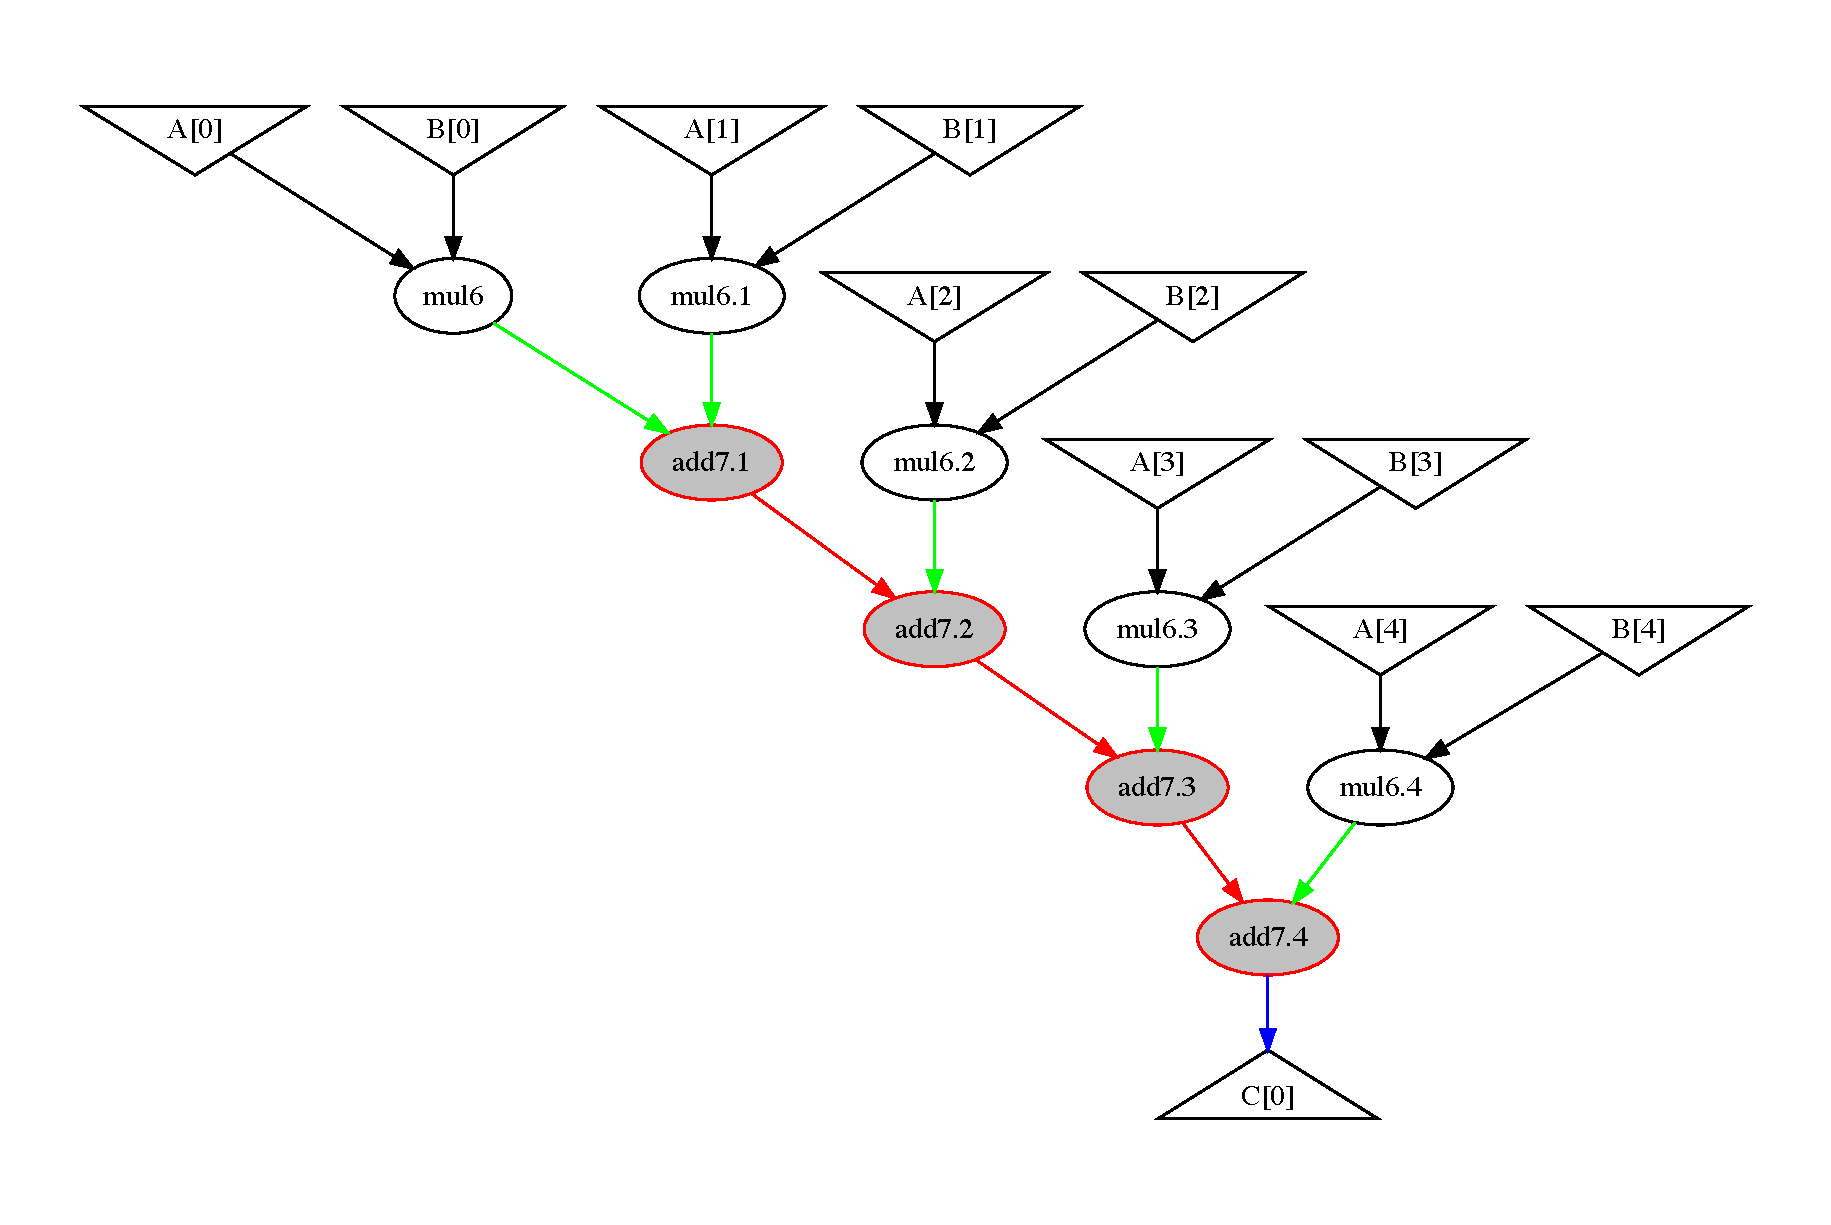
\includegraphics[width=.9\columnwidth,left]{images/supernode_2.pdf}
\caption{\small A Data Dependency Graph: inverse triangles represent input data, obtained from the \textit{load} instructions; ovals describe operations on data; the triangle at the bottom represents the result, derived from a \textit{store} instruction. Highlighted, a chain of associative operations before being optimized by the \textit{DDA} module (\ref{ssec:dda}).}
\label{fig:ddg}
\end{figure}

%This next paragraph might be replaced with a reference, we are interested mainly in the concept of mobility
Next, we apply the ASAP and ALAP scheduling methodologies\cite{hwang1991formal} to the generated DDG. These schedules will associate to each DDG node a clock cycle where the instruction is executed, and \textit{bound} the design space of possible architectures by determining the \textit{maximally parallel} architectures. We start by scheduling the input nodes of the DDG using the arrival clock time of their input data, computed as explained in Section~\ref{ssec:l2_read_model}, thus taking into account the L2M - L1M transfer time. Next, we determine the minimal latency required to obtain the outputs of the application with the ASAP schedule: starting from the DDG input leafs, each instruction node is scheduled as soon as its dependencies are resolved.
Once ASAP is completed, we can perform the ALAP scheduling: starting from the output leaf nodes, each node is scheduled as late as possible according to its dependencies. Once ALAP is completed, every node is annotated with an ASAP clock cycle and an ALAP one. The difference between these two clock cycles, called instruction \textit{mobility}, identifies an interval in which the instruction can be scheduled without changing the overall latency of the application.

The final stage of the \textit{Data Dependency Analysis} module will allocate the DDG nodes to PEs, leveraging the nodes mobility to minimize the number of PEs of the final hardware architecture.

\vspace{-2mm}
\subsection{PE allocation with Modified Interval Partitioning}
\label{ssec:modified_interval_partitioning}
\vspace{-1mm}
To generate a hardware architecture behaviorally equivalent to the input application and with the latency identified during the ASAP-ALAP scheduling, there are two main requirements: (1) each instruction needs to be computed within its ASAP-ALAP interval, and (2) instructions in the DDG which are executed by the same PE cannot be scheduled at the same time.
Our Modified Interval Partitioning (MIP) algorithm - based on the original greedy Interval Partitioning algorithm~\cite{greedyIntervalPartitioning} - is designed to generate, from a DDG, hardware architectures that meet both requirements. Listing~\ref{lst:modified_interval_partitioning} presents MIP, in pseudo-code. The original Interval Partitioning problem addresses the issue of assigning a number of jobs, with known starting and ending time, to the minimum amount of resources, ensuring that the jobs assigned to a resource do not overlap. To use Interval Partitioning for our problem, we consider instructions as jobs and PEs as resources. There are, however, three main differences between our problem and the canonical Interval Partitioning.
\begin{enumerate}
\item The original algorithm considers any job can use any resource, while our architecture requires different PEs for different instructions. We therefore perform interval partitioning several times (lines 5-20), once for each instruction type (e.g., four times for the graph in Figure \ref{fig:ddg}). This ensures a correct allocation of instructions to PEs performing the same operation.
\item Due to \textit{mobility}, instructions do not have a fixed starting time. MIP takes the mobility of an instruction into account by allowing a given instruction to start at any time within its allowed interval (lines 11-13).
\item Our instructions are dependent on each other, which is not the case for the jobs in the original interval partitioning. To account for this extra constraint, we ensure that any given instruction (a) is only allocated after its dependencies are allocated (line 4), and (b) is scheduled to start after the ending time of its dependencies (line 7-8).
\end{enumerate}
%Listing~\ref{lst:modified_interval_partitioning} presents MIP, in pseudo-code. %of our modified interval partitioning algorithm.

\begin{lstlisting}[language=Python, caption={\small Modified Interval Partitioning (MIP) Algorithm}, label={lst:modified_interval_partitioning}, basicstyle=\tiny]
# ASAP[i] and ALAP[i] contain the scheduled cycles for instruction i
# SetPEs is the set of Processing Elements in the architecture
SetPEs=[]
sort instructions by ASAP[i]
for each instruction i
	allocated = False
	dep_deadline = maximum end-time of all instructions depending on i
	schedule[i] = max(ASAP[i], dep_deadline)
	for each PE in SetPEs
		if instruction i matches PE
			if ALAP[i] >=  next_free_slot[PE]
				add instruction i to PE
				schedule[i] = max(schedule[i], next_free_slot[PE])
				next_free_slot[PE] = schedule[i] + latency(i)
				allocated = True
	if not allocated
		create new PE with type(i)
		add instruction i to PE
		next_free_slot[PE] = schedule[i] + latency(i)
		add PE to setPEs
\end{lstlisting}

%We assume that ASAP and ALAP schedules have been previously performed, hence we can have two data structures that return the ASAP and ALAP schedules for a given instruction i - i.e. ASAP[i] and ALAP[i].
%Instructions is an ordered list of instructions initialized with the instructions of the input application.
%A Functional Unit is represented as a set containing the instructions that have been allocated to it, and FunctionalUnits is a set containing the Functional Units of the resulting architecture which is initialized as an empty set.
%The functions latency and dep take an instruction i as input and return respectively the latency of i and a list of instructions i depends on.
%The function type takes as input a Functional Unit or an Instruction and returns the type of operation performed.

The MIP algorithm returns \verb|setPEs| and a \verb|schedule| for the current design: \verb|setPEs| is the list of processing elements that form the architecture, with each PE containing the instructions it has to execute, while \verb|schedule| contains the clock cycle at which each instruction is scheduled to be executed.

\vspace{-1mm}
\subsection{Most Parallel and Most Sequential Architectures}
\vspace{-1mm}
The result of the \textit{DDA} module is the \textbf{Most Parallel Architecture (MostPar)}. This architecture takes full advantage of the parallelism of the application and performs the computation with the minimum latency. However, MostPar uses the maximum number of PEs - in the worst case scenario equivalent to the number of instructions in the application - and it will hence have the largest area.
At the other end of the spectrum of architectures we can imagine the \textbf{Most Sequential Architecture (MostSeq)}, where no parallelism is used and the instruction are scheduled sequentially respecting their dependencies. This architecture will have the worst possible latency, but the minimal impact in area - using only one PE per operation type.
Probably none of these two architectures will be of direct interest for the user as they represent two extreme cases. Instead, the interesting architectures are the ones \textit{in between} \textbf{MostSeq} and \textbf{MostPar}, because they offer interesting trade-offs between power, latency and area. Section~\ref{ssec:dse} describes how these intermediate architectures can be generated using \textbf{MostPar} and \textbf{MostSeq} respectively as upper and lower bounds of the design space.

\section{\frameworkname: Design Space Exploration (DSE)}
%\vspace{-1mm}
%\subsection{Design Space Exploration}
\label{ssec:dse}
%\vspace{-1mm}
The \textit{Design Space Exploration} \frameworkname~module generates hardware architectures, behaviorally equivalent to the input application, which exhibit area, latency and power tradeoffs.
Our DSE - described in Listing \ref{lst:dse} - is an iterative process which produces, at the end of each iteration, a different hardware architecture.
The iterative process starts its sweep from \textbf{MostPar}, and ends when \textbf{MostSeq} is generated.
\begin{lstlisting}[language=Python, caption={\small Design Space Exploration},label={lst:dse},basicstyle=\tiny]
currentArchitecture = MostPar
found_MostSeq=False
GeneratedArchitectures=[]
while(!found_MostSeq)
    type_count={}
    found_MostSeq=True
    for each PE in currentArchitecture
        type_count[type(PE)]+=1
            if type_count[type(PE)] > 1
                found_MostSeq=False
                break
    if found_MostSeq
       break
    for each instuction i in DDG
        if type(i) == 'store'
            ALAP[i] = ALAP[i]+1
    ALAP=performALAPschedule(instructions,dependencies)
    SetPEs=MIP(instructions,ASAP,ALAP)
    GeneratedArchitectures+=[SetPEs]
    currentArchitecture=SetPEs
\end{lstlisting}
An iteration consists of three steps. First, the instructions corresponding to output leaf nodes in the DDG are selected. The ALAP schedule of these iterations is increased by 1 (lines 14-16), and the ALAP scheduling of the rest of the nodes in the DDG is updated accordingly (line 17). Consequently, the mobility of each instruction node is increased by one. Finally, the MIP is ran again (line 18), using the new ALAP schedule. Due to the increased mobility of each instruction the generated architecture is likely to use less PEs.
The process stops as soon as one iteration generates \textbf{MostSeq}, which can be recognized because it contains only one PE per operation type (lines 6-13).

There are two side benefits of our DSE approach. First, the user can tune the granularity of the exploration: by increasing the ALAP "slack" beyond 1, the exploration speeds-up, but less architectures are generated. Second, the DSE process can be easily parallelized, because its iterations are independent.

%This has been merged with the L2 Memory Read section
%\vspace{-1mm}
%\subsection{L2 Memory Write}
%\vspace{-1mm}
%The schedule produced by MIP includes the L2M-L1M transfer, and the computation; it does not include the L1M-L2M transfer. However, due to MIP, we do know the clock cycle at which computation ends (phase 2 in Figure~\ref{fig:system}) and the last data item is written in L1M. The L1M-L2M transfer can start immediately after the last output is generated.
%The latency of the L1M-L2M transfer is calculated using (2),
%\begin{equation}
%    WBL_{L2M} = S_w + W_{L2M} * O * \frac{B_{L2M}}{B_{L1M}} * \frac{Clk_{L1M}}{Clk_{L2M}}
%\end{equation}
%where the symbols have been defined in Table~\ref{table:equation}


\vspace{-1mm}
\subsection{Architecture Tradeoffs}
\label{ssec:arch_tradeoffs}
\vspace{-1mm}
%In section~\ref{
For a given input application and a given configuration, \frameworkname~outputs a set of hardware architectures - composed of spatial processor and L1M - with different area and latency trade-offs. Figure~\ref{fig:tradeoffs} shows three of the architectures generated during the DSE. Each box represents a PE. The different load and store PEs are implemented as separate L1M banks. As an example, the architecture in Figure \ref{fig:inter_arch} has 1 L1M bank to store the input data and 5 banks to store the results. This architecture can therefore receive 1 input element per clock cycle from the L2M, and store up to 5 results per clock in the L1M store banks. The remaining PEs are obtained from computing instructions. We allow the architectures to have cycles because the circuit is synchronous, and every instruction has been carefully scheduled. A self-loop in a PE indicates data reuse (see Section~\ref{sec:arch_template} for implementation details).
\begin{figure}[ht]
\centering
\begin{subfigure}{.4\columnwidth}
  \centering
  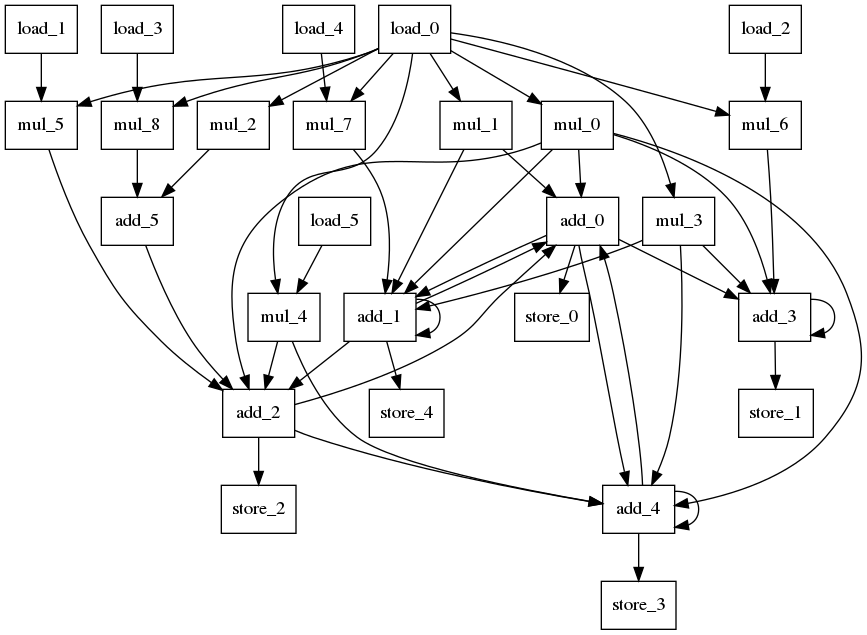
\includegraphics[width=\textwidth]{images/Architecture_latency_146_schematic.png}
  \caption{}
  \label{fig:max_par_arch}
\end{subfigure}%
\begin{subfigure}{.3\columnwidth}
  \centering
  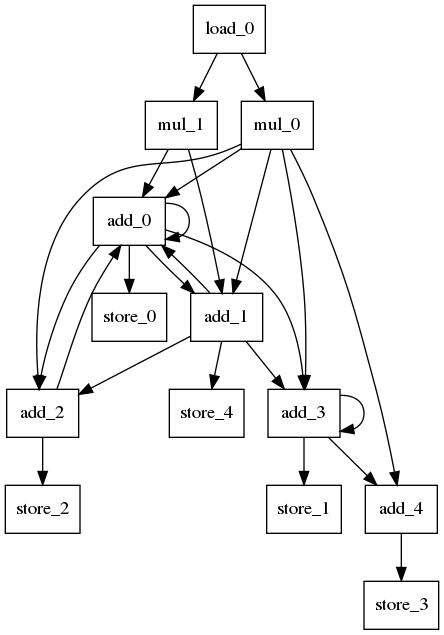
\includegraphics[width=\textwidth]{images/Architecture_latency_166_schematic.png}
  \caption{}
  \label{fig:inter_arch}
\end{subfigure}
\begin{subfigure}{.2\columnwidth}
  \centering
  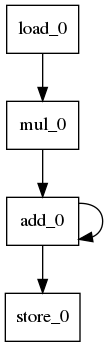
\includegraphics[width=0.5\textwidth]{images/Architecture_latency_188_schematic.png}
  \caption{}
  \label{fig:most_seq_arch}
\end{subfigure}
    \caption{\small Example of architectures generated from a matrix vector multiply application of size 5x5. The MostPar (a), an intermediate architecture (b) and the MostSeq (c).}
\label{fig:tradeoffs}
\end{figure}


\subsection{Multi-Configuration Design Space Exploration}
\label{ssec:multiconf_dse}
\frameworkname~can also perform design space exploration on the configuration parameters (Section~\ref{ssec:conf_param}), generating one configuration file for each combination of configuration parameters and aggregating the architectural trade-offs. This allows, as an example, to estimate the effect that different clock frequencies or different memory technology have on the area,latency and energy trade-offs. The use cases discussed in \ref{ssec:case_study2} and \ref{ssec:case_study3} are examples of multi-configuration DSEs.
%\begin{figure}
%
%\begin{minipage}{.5\linewidth}
%\centering
%\subfloat[]{\label{main:a}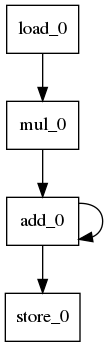
\includegraphics[scale=.2]{images/Architecture_latency_188_schematic.png}}
%\end{minipage}%
%\begin{minipage}{.5\linewidth}
%\centering
%\subfloat[]{\label{main:b}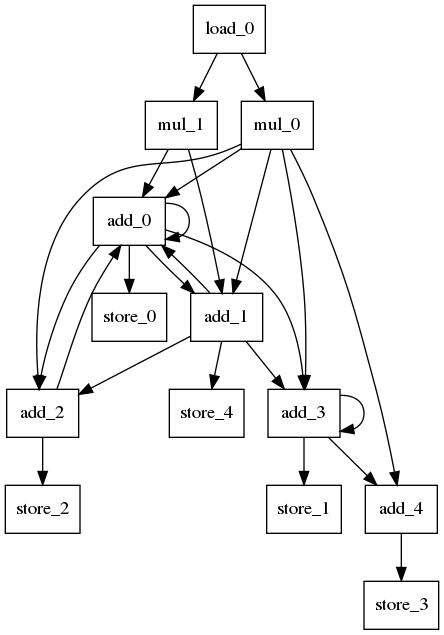
\includegraphics[scale=.2]{images/Architecture_latency_166_schematic.png}}
%\end{minipage}\par\medskip
%\centering
%\subfloat[]{\label{main:c}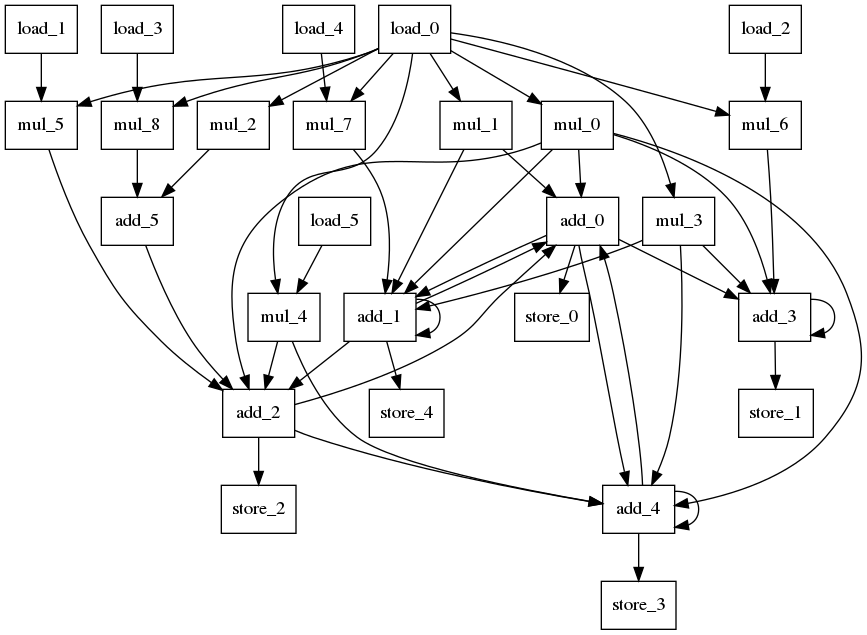
\includegraphics[scale=.10]{images/Architecture_latency_146_schematic.png}}
%
%\caption{my fig}
%\label{fig:main}
%\end{figure}
